\chapter{Introducción}\label{cap.introduccion}
En este primer capítulo se explica el contexto de las bases tecnológicas en las que se apoya este proyecto, que son principalmente las tecnologías web y la robótica. Para empezar se habla sobre el estado actual de la robótica y la gran expansión de la misma en nuestros días. Se continúa señalando el contexto de las tecnologías web y como de importantes son en la sociedad actual, para continuar explicando su arquitectura y las tecnologías más importantes. Para finalizar este capitulo, se introducen proyectos previos que combinan tecnologías web con componentes robóticos.

\section{Robótica}
El diccionario de la Real Academia Española define robótica como la técnica que aplica la informática al diseño y empleo de aparatos que, en sustitución de personas, realizan operaciones o trabajos, por lo general en instalaciones industriales. 

Desde que Asimov acuñara sus tres leyes, la sociedad ha temido lo que los robots puedan hacer al ser humano, desde esclavizarnos hasta quitarnos el trabajo, siendo este miedo el más reciente. Sin embargo, con el paso del tiempo, nos hemos dado cuenta que la robótica tiene una gran utilidad para hacer avanzar la sociedad. Ya no solo pensamos en robótica como en un humanoide que pueda reemplazar al ser humano como nos muestran tantas obras literarias y cinematográficas, sino que vemos robótica a lo largo de nuestro día a día, desde un brazo mecánico en una cadena de montaje, hasta un aspirador robótico. Tareas que hasta hoy conllevaban riesgos para la salud humana como la desactivación de artefactos explosivos o trabajos con altas temperaturas, o tareas pesadas y repetitivas se pueden realizar de manera más eficiente y fácil gracias a la robotización de las mismas.

\subsection{Productos e investigación robitca}
El uso de la robótica en la actualidad está muy extendido, tareas tales como montajes en cadena en una fabrica, trabajos repetitivos de gestión de proyectos o manipulación de objetos peligrosos, ya están robotizados de manera que el ser humano no se ponga en peligro o malgaste tiempo de manera innecesaria. A continuación se muestran varios ejemplos de uso de la robótica en nuestros días:
\begin{itemize}
\item Cirugía: Los robots se están empezando a usar en procedimientos quirúrgicos, ya que compensan las deficiencias y limitaciones del ser humano en la exactitud y precisión. Además, posibilitan la ``telecirugía'', que se trata de la realización de intervenciones quirúrgicas de manera remota mediante brazos robóticos que imitan al milímetro los movimientos de un cirujano situado en cualquier lugar. La primera ``telecirugia'' fue realizada en el año 2001 por cirujanos estadounidenses que operaron a un paciente en Francia y ha supuesto una revolución en la medicina, al poder realizar intervenciones quirúrgicas separadas por miles de kilómetros. Actualmente, ya se comercializan sistemas como el Da Vinci pensado para mejorar la laparoscopia, permitiendo al cirujano operar sentado y visualizando en un monitor la imagen del paciente, proporcionando una mayor precisión al evitar los temblores, mejor visualización y mayor destreza.
\begin{figure}[H]
  \begin{center}
    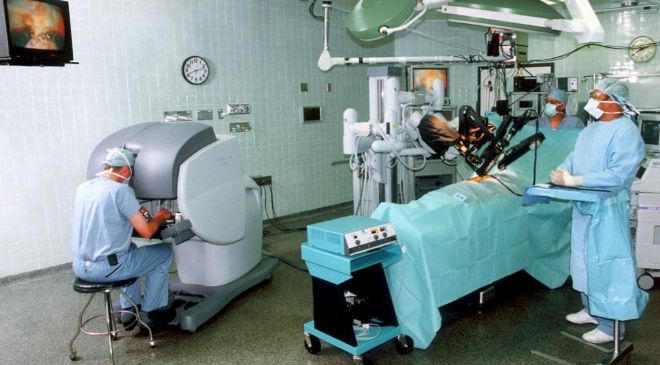
\includegraphics[width=0.8\textwidth]{figures/sistemadavinci.jpg}
		\caption{Sistema Da Vinci}
		\label{fig.sistemadavinci}
		\end{center}
\end{figure}
\item Industria: Es el sector donde más extendido este el uso de la robótica, desde mover una pieza de posición hasta cargar y descargar máquinas. Hay una donde sobresale por encima del resto: el sector del automóvil. En España, según datos de la Asociación Española de Robótica, seis de cada diez robots pertenecen a este sector. Los robots se encargan de distribuir por toda una fabrica los componentes necesarios, así como posteriormente montarlos. Gracias a la robotización de la industria, la producción ha aumentado en los últimos años de manera significativa, disminuyendo costes y errores.
\begin{figure}[H]
  \begin{center}
    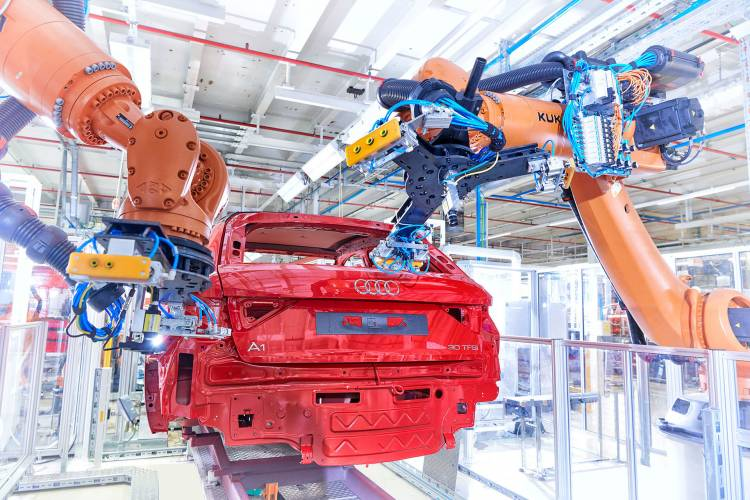
\includegraphics[width=0.8\textwidth]{figures/robotautomovil.jpg}
		\caption{Fábrica de Seat en Martorell}
		\label{fig.robotautomovil}
		\end{center}
\end{figure}
\item Militar: El sector militar es donde más dinero se invierte y se investiga. Actualmente hay multitud de robots usados militarmente como los vehículos aéreos no tripulados Hermes y Predator, el Goalkeeper CIWS, que es un sistema de armamento defensivo por proximidad holandés, o Samsung SGR-A1, que es un robot centinela utilizado para la vigilancia de la zona desmilitarizada entre Corea del Sur y Corea del Norte. Se está investigando la elaboración de un robot humanoide capaz de caminar por terrenos irregulares y zonas catastróficas para realizar tareas de rescate y ayuda humanitaria. En este sentido, entre el año 2012 y 2015, el Departamento de Defensa de Estados Unidos, a través de su Agencia de Proyectos  de Investigación Avanzada en Defensa (DARPA), creó una competición con el objetivo de desarrollar robots terrestres semiautónomos capaces de realizar tareas complejas en entornos peligrosos y degradados\footnote{\url{https://www.darpa.mil/program/darpa-robotics-challenge}}. El premio fue ganado por el robot humanoide desarrollado por el Instituto Avanzado de Ciencia y Tecnología de Corea, ``DRC-Hubo'' (figura 1.3).
\begin{figure}[H]
  \begin{center}
    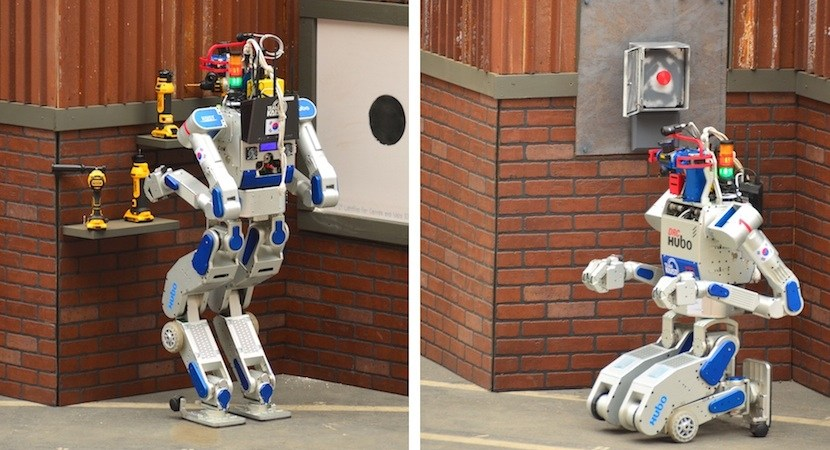
\includegraphics[width=0.8\textwidth]{figures/drchubo.jpg}
		\caption{Robot DRC-Hubo durante el DARPA Robotics Challenge}
		\label{fig.drchubo}
		\end{center}
\end{figure}
\end{itemize}

\subsection{Software para robots}
Todo robot tiene una parte hardware (el componente robótico ya sea real o simulado) y una parte software (la lógica de ese componente robótico).

El software es el encargado de proporcionar al robot la inteligencia y autonomía necesaria para que realice las funciones o acciones que deseamos. Para facilitar esta tarea, se han creado middleware y bibliotecas especificas.

Un middleware  proporciona las herramientas que se necesitan para facilitar el desarrollo de software robóticos, ya que permite estructurar el software separando las diferentes tares (lectura de sensores, extracción de datos, especificar la velocidad, etc.) y haciendo exportable el uso de este software con cualquier otro sistema robótico al tener un marco común de comunicación gracias al middleware.
Actualmente hay una gran cantidad de middleware que permiten esta abstracción, siendo algunos de los más destacados los que señalo a continuación:
\begin{itemize}
	\item Robot Operating System (ROS)\footnote{\url{http://www.ros.org/}}: Provee de la funcionalidad que cabría esperar de un sistema operativo (abstracción del hardware, control de dispositivos de bajo nivel, la trasferencia de mensajes entre procesos, administración de paquetes, etc.). El principal objetivo es permitir la reutilización del código en la investigación y desarrollo de robótica, lanzando paquetes de software que están listos para ser usados por cualquier desarrollador. ROS cuenta con una gran comunidad de colaboradores, que comparten sus paquetes y proyectos, gracias a su sitio web y repositorios.
	\item Open Robot Control Software project (Orocos)\footnote{\url{http://www.orocos.org/}}: Se trata de un proyecto de software libre cuyo objetivo es la creación de un paquete de software para el control de robots.
	\item JdeRobot\footnote{\url{https://jderobot.org/}}: Se trata de una plataforma de código abierto para el desarrollo de aplicaciones de visión artificial y robóticas, compatible con middlewares de comunicación ICE y ROS y desarrolladas principalmente en Python y C++. 
\end{itemize}

Hay multitud de bibliotecas para el desarrollo de sistemas robóticos: bibliotecas para procesar imágenes, interactuar con el robot, procesar elementos 3D, etc. Algunas de las bibliotecas más utilizadas son:
\begin{itemize}
	\item OpenCV\footnote{\url{https://opencv.org/}}: Es la biblioteca de visión artificial por excelencia. Creada originalmente por Intel, es de código abierto y desarrollada en C++. Actualmente dispone de interfaces en C++, C, Python, Java y están empezando a desarrollar para JavaScript.
	\item Point Cloud Library (PCL)\footnote{\url{http://pointclouds.org/}}: Se trata de una biblioteca de código abierto que proporciona algoritmos para el procesamiento de nubes de puntos y geometría 3D.
	\item Bibliotecas de ROS: ROS proporciona bibliotecas para cada lenguaje de programación al que da soporte, ofreciendo una serie de funciones y algoritmos que nos permite crear aplicaciones que interactúan rápidamente con ROS. Las bibliotecas más utilizadas son \texttt{rospy}\footnote{\url{http://wiki.ros.org/rospy}}, desarrollada para Python y \texttt{roscpp}\footnote{\url{http://wiki.ros.org/roscpp}}, desarrollada para ser usada con C++. Cabe destacada, también, la biblioteca \texttt{roslibjs}, que ofrece las funcionalidades para JavaScript.
\end{itemize}

Finalmente, cabe mencionar los simuladores robótico, que imitan el funcionamiento de un sistema robótico para probar las aplicaciones, evitando que surjan fallos críticos a la hora de hacerlo funcionar con el sistema real. Estos fallos pueden conllevar averías muy costosas a nivel monetario y de tiempo, que conllevarían retrasos importantes a la hora de realizar el desarrollo. 

El simulador más utilizado es Gazebo\footnote{\url{http://gazebosim.org/}} gracias a su fácil manejo y su intuitiva interface. Gazebo es un simulador de código abierto que ofrece múltiples motores de físicas, motores de renderizado avanzado, soporte para plug-ins y programación en la nube. Además, dispone de un gran número de robots, sensores y cámaras para simular, lo que permite realizar las pruebas de nuestras aplicaciones de forma bastante realista y, así poder utilizar nuestra aplicación con el sistema físico sin miedo a que sufra daños.

Existen otros simuladores como Stage\footnote{\url{http://rtv.github.io/Stage/index.html}} para la simulación en 2D o Webots\footnote{\url{https://www.cyberbotics.com/}}.

\section{Tecnologías web}
Desde que en el año 1992, Tim Berners-Lee ideara y desarrollara las primeras herramientas para facilitar compartir información entre los científicos del CERN desde cualquier parte del mundo, dando lugar a la posteriormente llamada World Wide Web o como se conoce coloquialmente la web, ha sufrido una gran evolución, consiguiendo que la sociedad actual no se pueda entender sin la existencia de la misma. Sin embargo, pese a la gran evolución, el propósito de la web no ha cambiado, es decir, que acceder a la información sea lo más fácil posible. Sí lo ha hecho la manera en se utiliza. La aparición de aplicaciones web como las redes sociales, los servicios de streaming o los comercios electrónicos, han supuesto un impulso importante en el uso de la web y la necesidad de idear nuevas herramientas que faciliten el desarrollo de webs.

 A continuación se muestran algunos ejemplos de aplicaciones y páginas web muy utilizadas:
\begin{itemize}
\item Spotify\footnote{\url{https://www.spotify.com/es/}}: Aplicación creada para la reproducción de música vía streaming, actualmente cuenta con más de 75 millones de usuarios activos siendo una de las principales formas de escuchar música en la actualidad. La aplicación esta desarrollada mediante JavaScript (lado del cliente) y Python (lado del servidor).
\item Netflix\footnote{\url{https://www.netflix.com/es/}}: Comenzó como un videoclub donde se alquilaban DVDs a través de una página web y se enviaban por correo postal, para pasar a proporcionar un servicio de video bajo demanda por internet. Cuenta con más de 110 millones de usuario suscritos a su servicio y ha supuesto una revolución al cambiar el modo en que la sociedad ve contenidos audiovisuales, gracias a su facilidad de uso mediante su aplicación web. Este auge ha llevado a Netflix, con el fin de nutrir a sus suscriptores del máximo contenido posible, a realizar sus propias producciones. 
\item Facebook\footnote{\url{https://es-es.facebook.com/}}: La red social más conocida y que provoco el auge de las mismas, actualmente cuenta con más de 2200 millones de usuarios. Originalmente nació como una página web desarrollada mediante HTML y JavaScript para el lado del cliente y PHP para el lado del servidor, ha evolucionado hasta disponer una aplicación que puede ser utilizada en nuestros teléfonos móviles.
\item Google maps\footnote{\url{https://www.google.es/maps}}: Un servicio de mapas que permite desplazarse por el mundo, ver fotografías por satélite o recorrer una ubicación a pie de calle. Actualmente es utilizada para indicar ubicaciones, a modo de GPS o para encontrar lugares de interés. La base de esta aplicación es JavaScript, usando HTML y CSS para la interfaz gráfica.
\item YouTube\footnote{\url{https://www.youtube.com/}}: Aplicación y página web dedicada a la compartición de videos entre usuarios. Actualmente cuenta con más de 1900 millones de usuarios al mes y cada minuto se suben más de 120 horas de vídeo, llegando a convertirse en un oficio para miles de personas que ganan dinero publicando sus propios videos comentando videojuegos, consejos o criticas de multitud de cosas (móviles, películas, juguetes, etc.). YouTube está desarrollado mediante JavaScript y HTML en el lado del cliente y Python en el lado del servidor, incluso proporciono el primer reproductor de video incrustado en el HTML, que posteriormente fue incluido por el World Wide Web Consortium.
\item Whatsapp\footnote{\url{https://www.whatsapp.com/}}: Es una aplicación de mensajería instantánea que permite el intercambio entre usuarios de mensajes a través de internet sin coste adicional. Cuenta con más de mil millones de usuarios. Ha supuesto una revolución al provocar la extinción del servicio de mensajes cortos (SMS) que conllevaban un coste mensual alto en beneficio de las operadoras móviles. Tras ser usado como aplicación en teléfonos móviles, en el año 2015 se lanzó la versión web de Whatsapp para su uso en un ordenador, provocando que la aplicación de mensajería de Google, Hangouts, sufriera una reducción importante de usuarios, siendo uno de los factores que ha llevado a Google a anunciar el cierre del servicio en el año 2020.
\end{itemize}

\subsection{Arquitectura de una aplicación web}
Desde su creación, el modelo para que un sitio o aplicación web funcione no ha variado.
\begin{itemize}
	\item Cliente: Realiza las peticiones de recursos a diferentes servidores web a través de un localizador uniforme de recursos (URL). Generalmente, la función de cliente la realizada un navegador.
	\item Servidor: Almacena la información de la aplicación web y sirve los contenidos acorde a las peticiones realizada por el navegador.
	\item Http: Es el protocolo permite el intercambio de información entre el cliente y el servidor.
\end{itemize}
\begin{figure}[H]
  \begin{center}
    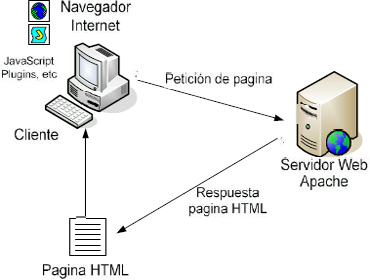
\includegraphics[width=0.8\textwidth]{figures/arquitecturaweb.jpg}
		\caption{Arquitectura de una aplicación web}
		\label{fig.arquitecturaweb}
		\end{center}
\end{figure}

\subsection{Tecnologías del lado del cliente}
Estas tecnologías son las encargadas de dar forma a la interfaz de usuario y de establecer la comunicación con el servidor. El navegador es capaz de leer e interpretar estas tecnologías. Las más utilizadas son las siguientes:
\begin{itemize}
	\item Hyper-Text Markup Lenguage (HTML): Es el lenguaje de descripción de aplicaciones web que nos permite especificar las características visuales. Actualmente se utiliza la quinta revisión llamada HTML5, que aporta una gran mejora como son las etiquetas para reproducir contenido multimedia.
	\item Hojas de estilo en cascada (CSS): Es el lenguaje utilizado para describir la presentación semántica (el aspecto y el formato) de un documento en lenguaje de marcas.
	\item JavaScript: Es un lenguaje de script orientado a objetos y guiado por eventos que nos permiten realizar acciones en el cliente e interactuar con el servidor u otras aplicaciones web.
\end{itemize}

\subsection{Tecnologías del lado del servidor}
Estas tecnologías son las encargadas de dar forma al servidor web de manera que permita el acceso a bases de datos, conexiones de red, recursos compartidos, en definitiva, se encarga de realizar todas las tareas necesarias para crear la aplicación web que se visualizará en el cliente. Las tecnologías más utilizadas son las siguientes:
\begin{itemize}
	\item PHP: Creado en 1994, es la tecnología más utilizada. Se trata de un lenguaje de programación de uso general de script que originalmente fue diseñado para proporcionar contenido web dinámico. Su código está empotrado en el código HTML y es interpretado por un servidor web para generar la aplicación web, evitando la necesidad de acceder a un archivo externo.
	\item Python, Django: Se trata de un framework programado en Python que proporciona un conjunto de componentes en el lado del servidor para ayudar a la hora de desarrollar una aplicación web. Sigue el diseño de Modelo-Vista-Controlador, que se trata de un modelo que separa la lógica y datos de la interfaz gráfica y de las comunicaciones y eventos. Cuando un cliente solicita una URL al servidor, esta pasa por Django que analizará la URL solicitada y pasará la petición a la función correspondiente llamada vista. En esta función se ejecutará lo necesario para proporcionar al cliente lo solicitado con su URL.
	\item Ruby on Rails: Al igual que Django, Ruby on Rails se trata de un framework para facilitar el desarrollador web programado en Ruby que sigue el diseño de Modelo-Vista-Controlador. El funcionamiento de Django y Rails es muy similar, siendo la principal diferencia el lenguaje en el que están programados, siendo necesario menos código en el caso de Rails.
	\item Node.js: Se trata de un entorno de ejecución multiplataforma de código abierto para el lado del servidor basándose en el lenguaje JavaScript. Este entorno se basa en eventos y gestiona todas las operaciones con una programación asíncrona. Todo esto facilita el desarrollo de aplicaciones web escalables de manera sencilla y con robustas.
\end{itemize}

\section{Tecnologías web en robótica}

La utilización de tecnologías web en robótica es aún un campo con poco desarrollo. Sin embargo, debido a las ventajas que ofrece frente a otras tecnologías (el mismo código funciona en cualquier plataforma, no es necesario realizar ninguna instalación, etc.) es un campo prometedor de cara al futuro.

Uno de los desarrollos más importante de tecnologías web en robótica son las bibliotecas y herramientas de código abierto para su utilización con el middleware ROS, elaboradas por la comunidad de Robot Web Tools\footnote{\url{http://robotwebtools.org/}}. Por ejemplo:
\begin{itemize}
	\item \texttt{Rosbridge Suite}: Proporciona una interfaz usando JSON para ROS que permite a cualquier cliente enviar JSON para conectarnos con el robot, mediante las capas de comunicación WebSockets, UDP y TCP. Realmente podría entenderse como un servidor intermedio que recibe o envía la información a un cliente web.
	\item \texttt{roslibjs}: Se trata de la biblioteca que da soporte a la interactuación entre una aplicación web desarrollada en JavaScript con ROS. 
	\item \texttt{ros2djs} y \texttt{ros3djs}: Son las bibliotecas elaboradas para gestionar la visualización de elementos en dos y tres dimensiones, respectivamente. Están elaboradas utilizando roslibjs y proporcionan funciones que son estándares en ROS como la elaboración de mapas, el procesado de nubes de puntos o del escaneo laser.
\end{itemize}

Adicionalmente Robot Web Tools, ofrece una serie de herramientas como son un servidor de video web, una herramienta para mostrar e interactuar con la navegación autónoma del robot, una herramienta para la creación de teleoperadores de robots, etc.

Otro ejemplo de desarrollos robóticos con tecnologías web son los TFGs realizados en el Grupo de Robótica de la URJC. Una parte de este proyecto está basado en el TFG elaborado por Aitor Martínez \footnote{\url{https://jderobot.org/Aitormf-tfg}}. En este trabajó se crearon tres aplicaciones que eran capaces de conectarse con varios sistemas robóticos: \texttt{CameraViewjs}, \texttt{KobukiViewerjs} y \texttt{UavViewerjs}.

\texttt{CameraViewjs} es un visualizador de imágenes, desarrollado utilizando JavaScript, HTML5 y CSS3 en el lado del Cliente y NodeJS en el lado del servidor, e ICE como middleware. Esta aplicación permite la visualización de las imágenes recibidas desde un servidor de imágenes, ya sean obtenidas desde una webcam, una cámara conectada a un robot o almacenadas en el dispositivo. En la figura 1.5 se puede ver el uso de esta aplicación

\begin{figure}[H]
  \begin{center}
    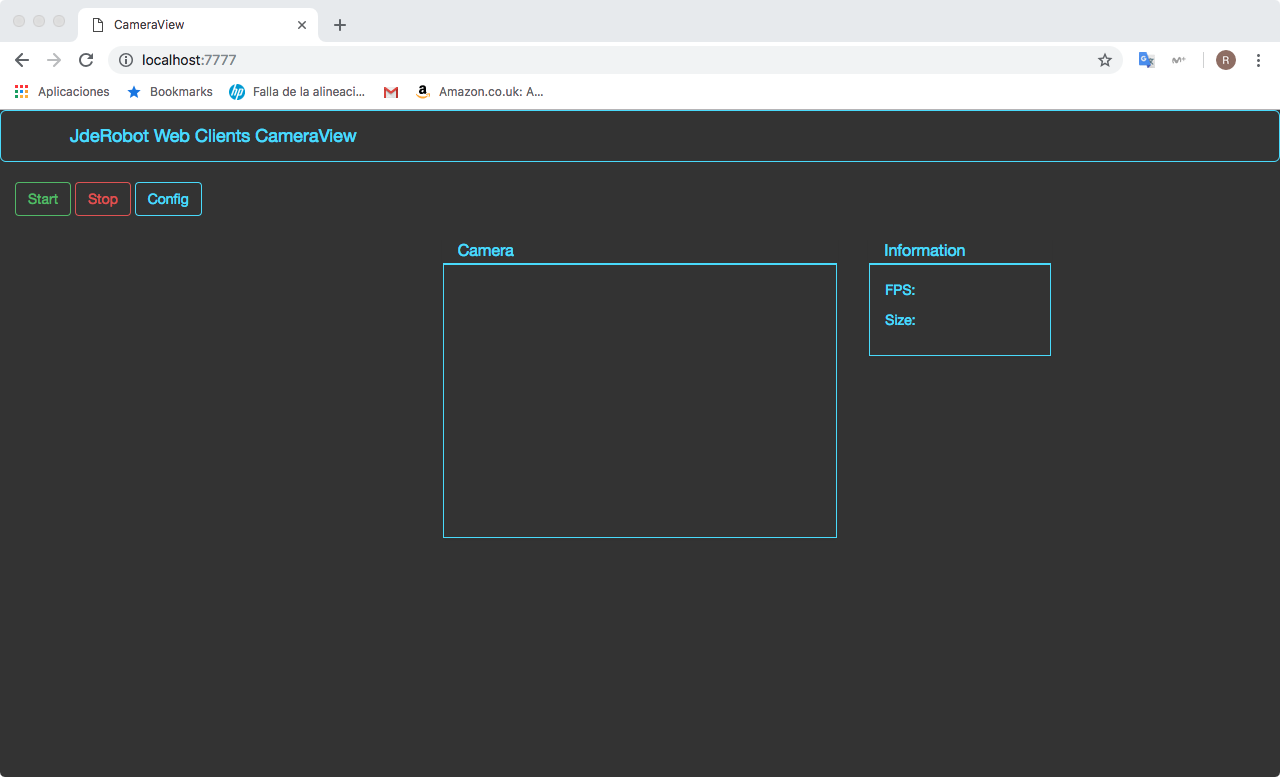
\includegraphics[width=0.8\textwidth]{figures/cameraviewjs.png}
		\caption{CameraViewjs}
		\label{fig.cameraviewjs}
		\end{center}
\end{figure}


\texttt{KobukiViewerjs} es un visualizador y teleoperador de robots del tipo Turtlebot, desarrollado utilizando JavaScript, HTML5 y CSS3 en el lado del Cliente y NodeJS en el lado del servidor, e ICE como middleware. Consta de varias partes, la primera de ellas es mostrar las imágenes obtenida a través de las dos cámaras de las que dispone el robot (izquierda y derecha), otra parte donde muestra la imagen del escaneo láser obtenida, una representación tridimensional del robot y el movimiento del mismo, y por último, el teleoperador, que envía al robot una velocidad lineal y otra angular para indicar tanto el movimiento en linear recta como la orientación del mismo. En la figura 1.6 se puede ver un ejemplo de uso de esta aplicación

\begin{figure}[H]
  \begin{center}
    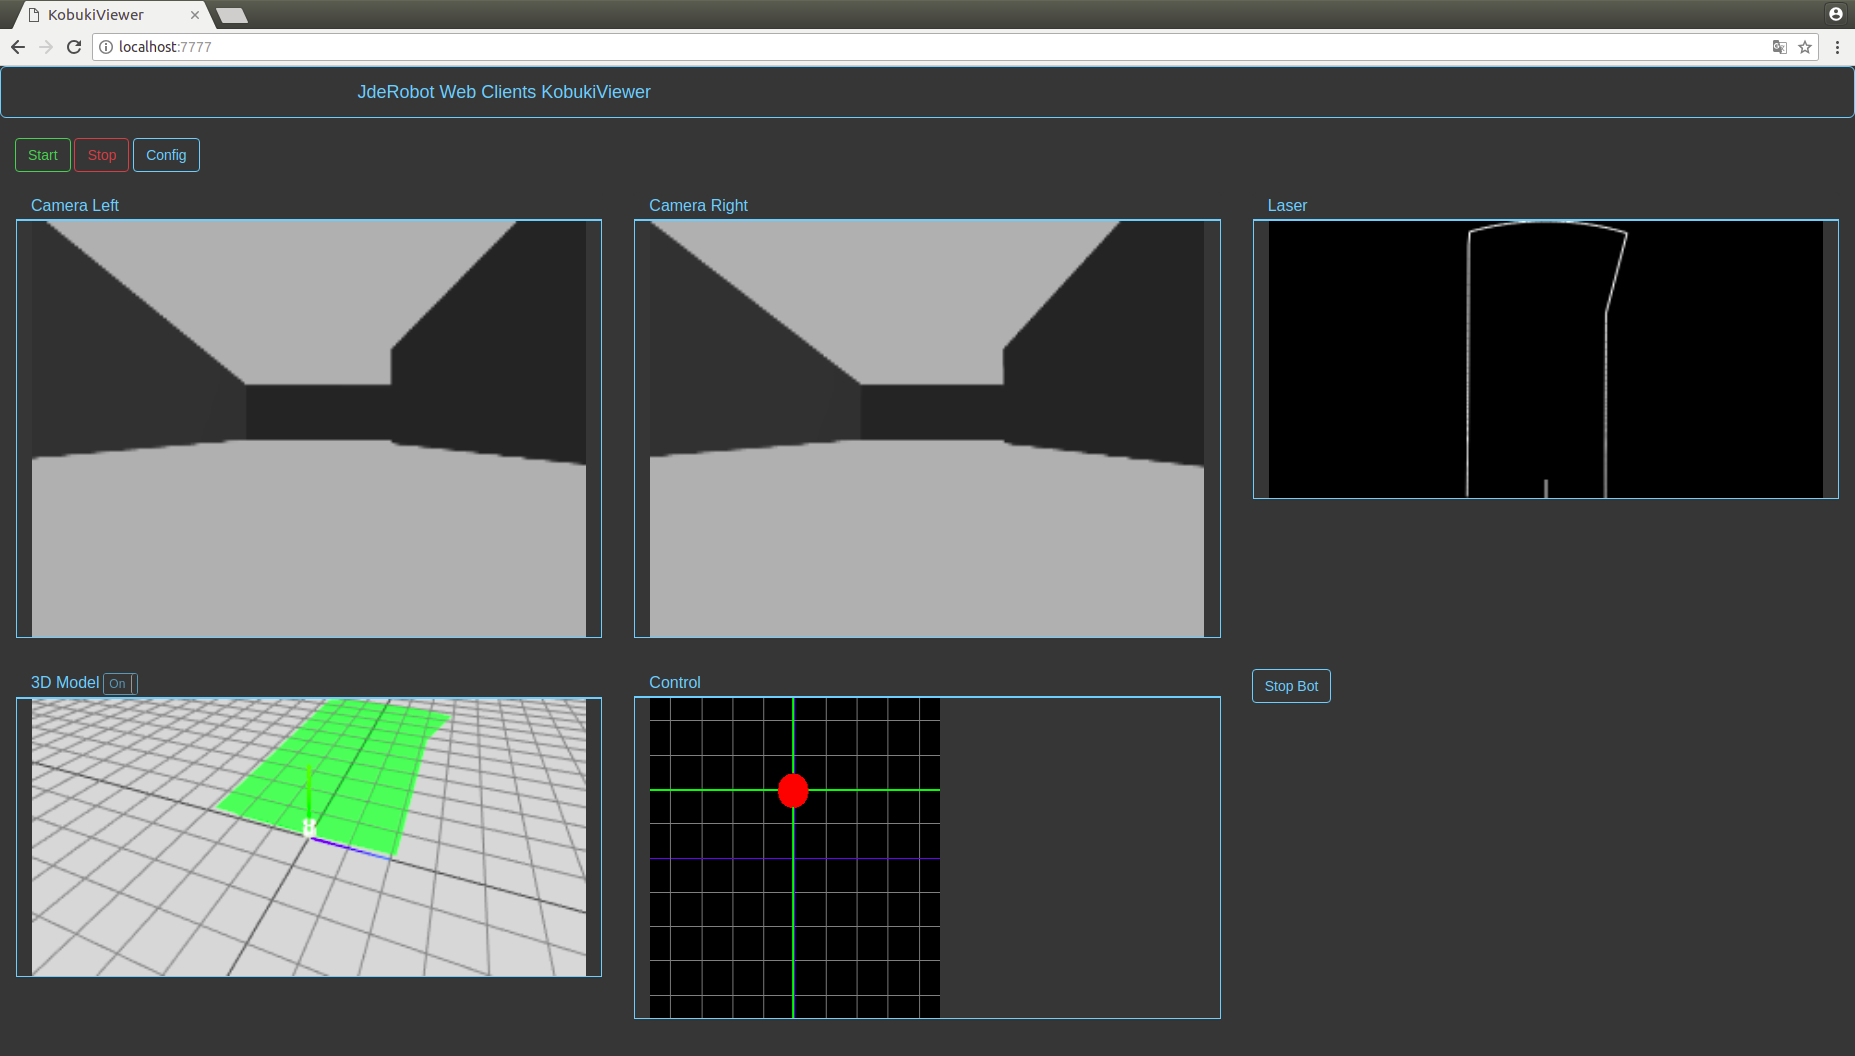
\includegraphics[width=0.8\textwidth]{figures/kobukiviewerjs.png}
		\caption{KobukiViewerjs}
		\label{fig.kobukiviewerjs}
		\end{center}
\end{figure}

\texttt{UavViewerjs} es un visualizador y teleoperador de drones, desarrollado utilizando JavaScript, HTML5 y CSS3 en el lado del Cliente y NodeJS en el lado del servidor, e ICE como middleware. La aplicación tiene integrada sobre la misma pantalla el teleoperador y la imagen obtenida de la cámara, pudiéndose elegir si deseamos mostrar la cámara frontal o de abajo del dron. Consta también de una representación tridimensional del dron y de su movimiento. Desde la aplicación se teleopera mediante él envió de una velocidad lineal y otra angular, además se le indica cuando se desea aterrizar y despegar. En la figura 1.7 se muestra una prueba de esta aplicación.

\begin{figure}[H]
  \begin{center}
    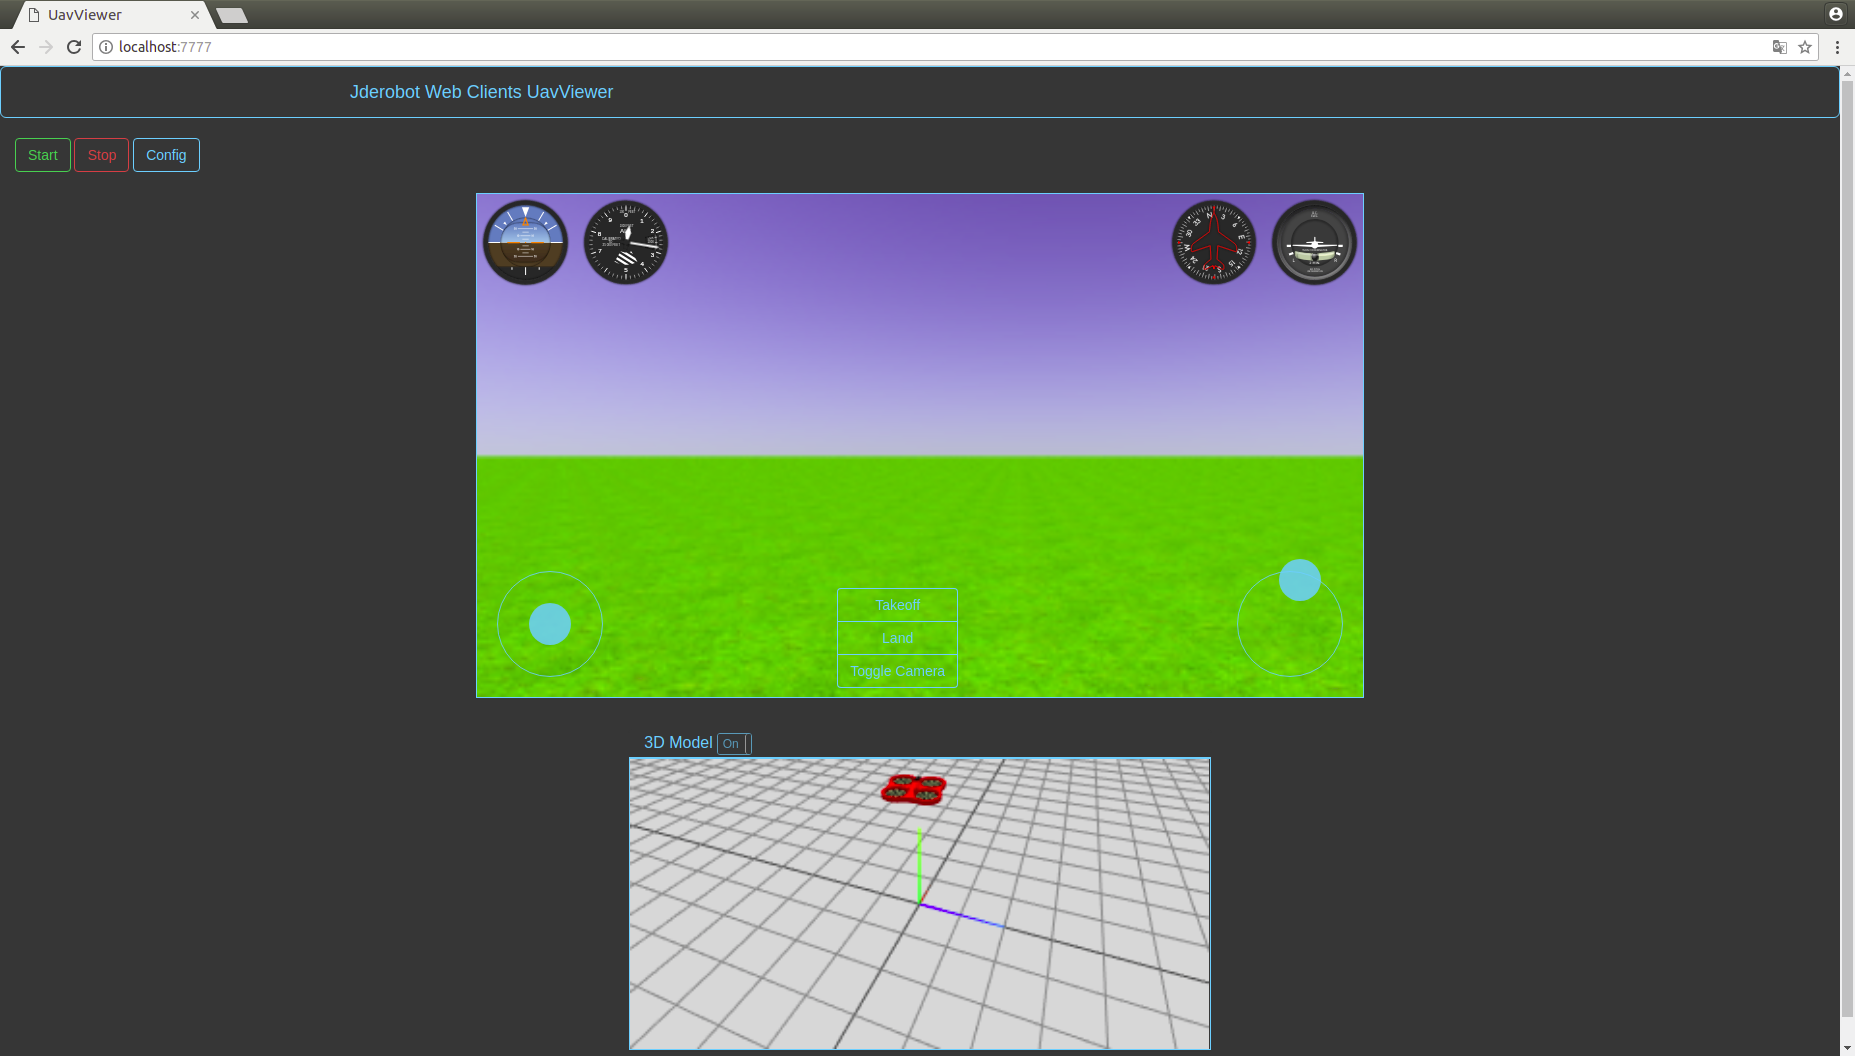
\includegraphics[width=0.8\textwidth]{figures/uavviewerjs.png}
		\caption{UavViewerjs}
		\label{fig.uavviewerjs}
		\end{center}
\end{figure}